\documentclass{article}

\usepackage{hyperref}
\usepackage{gensymb}
\usepackage{tipa}

\usepackage{svg}
\usepackage{graphicx}
\svgpath{{./images/}}
\graphicspath{{./images/}}

\newcommand{\w}{\super w}

\newcommand{\thetitle}{The Universe of the Kal People}
\newcommand{\theauthor}{Owen Bechtel}

\title{\thetitle}
\author{\theauthor}
\hypersetup{
  pdftitle={\thetitle},
  pdfauthor={\theauthor}
}

\begin{document}
\maketitle

\section{Introduction}

Hom, the world herein described, is inhabited by many peoples, including the Kal people, who speak the Kalvaszti language and live on a chain of islands known as Kalnot. The term \textit{Hom} is a transcription of the Kalvaszti word \textipa{/h\w om/} --- other peoples have different names for the world.

Hom is cosmologically very different from our own universe. For one thing, the world is flat and circular, rather than spherical. But the people that inhabit it are, in appearance and biology, identical to Earth humans. There are no elves, dwarves, goblins, or aliens. There are, however, gods and angels, as well as spirits of varying moral character; these interact with humans only rarely. There is no ``magic system,'' although supernatural things have been known to happen from time to time, and there are a few objects scattered throughout the world with peculiar properties. The Kal fight with guns and cannons, although this technology has not yet spread to much of the world. Men travel by horse and by sail. A Kal mathematician recently computed the value of $\sum_{n = 1}^\infty 1/n^2$, solving a century-old problem. Men in Kalnot and on the nearby mainland have begun to develop the very first steam engines.

The present age is an age of expansion for the Kal people. In the last few centuries, they have settled numerous previously-uninhabited islands throughout the ocean. About one hundred years ago, they first made contact with the vast continent of Terba across the sea, inhabited by many peoples formerly unknown to them. They are beginning to explore the interior, and are meeting some hostility from the native pastoralists.  

\section{Cosmology and Theology}

\subsection{Suns, Moons, and Ether Curtains}

There are two suns and two moons, which travel in circles above the world. To an observer on the ground, only one of these is visible at once, except at sunrise and sunset, when a sun and a moon are both dimly visible. To prevent the sun on the opposite side of the world from begin visible, there are four curtains of dark ether that rotate along with the suns and moons and divide the world into quadrants. Dark ether is a substance that interacts only with light and not with matter. A wider and/or denser curtain of dark ether will allow less light to pass through it. The ether curtains in Hom are just wide enough to prevent essentially all light from passing through them, so that the suns are not visible during the night. Sunset and sunrise --- the periods in which one is inside an ether curtain --- each last about 1/50 of a day, or 30 minutes. The length of a day on Hom is not significantly different from that of a day on Earth. ``Day'' in this context refers to a single day-night cycle, or half a rotation.

\begin{figure}[h]
  \centering
  \includesvg[width=6cm]{sun-moon}
  \caption{A diagram of Hom showing suns, moons, and dark ether. Not to scale. The suns and moons are not actually orange and blue.}
\end{figure}

In addition to the ether curtains, there are two other regions of dark ether: the inner darkness and the outer darkness. The inner darkness is a cylindrical region of dark ether in the center of the world. Below the inner darkness is a large, cold region of ocean that receives no natural light. The outer darkness surrounds the world and is of unknown thickness. It contains both land and ocean, but the ocean is frozen due to the very cold climate. (The outer regions of Hom are analogous to Earth's polar regions.) The ether of the outer darkness is less dense than that of the inner darkness, so the sun's light penetrates farther into the former. An explorer venturing into the outer darnkess would see the world around him become colder and darker day after day, until reaching a land of permanent moonless and starless night.

Like our own moon, the moons of Hom go through a cycle, but instead of changing shape, they simply vary in brightness while remaining circular. Hom's lunar cycle has a period of about 39.611 days. At their minimum brightness, the moons emit no light at all. At their maximum, they are as bright as a full moon on Earth.

\subsection{Stars}

The sky contains around 100,000 stars of varying luminosities. 90--95\% of these stars are not visible with the naked eye, and can only be seen with the use of a telescope or a similar device. Like on Earth, the stars are only visible at night due to the sun's much greater brightness. The stars orbit in the same direction as the suns and the moons (counterclockwise), but travel very slightly slower. Ignoring this difference in speed, the night sky alternates between two different sets of stars, as it takes two days for the sky to return to its original position. The tiny difference in speed between the stars and the moons has the effect that, after about 40 years, the moons will have rotated by one half turn relative to the stars, so the same set of stars will be visible once again, but under the opposite moon.

About once per century, a new star appears in the sky, or an existing one disappears. The folk religions of Hom have a variety of explanations for why this occurs, the most common being that a star is added when a great man dies, and removed when a great man is born.

It is important to remember that suns, moons, and stars are not of the same nature in Hom as they are in our universe. They are simply glowing orbs floating in the sky.

\subsection{Tides}

The amount of water in the ocean increases and decreases cyclically, causing the sea level to rise and fall in a manner analogous to Earth's tides. Unlike on Earth, high tide occurs at the same time all across the world, ignoring small differences caused by local geography. The tides are more extreme when the moons are brighter (spring tide), and less extreme when the moons are less bright (neap tide). The moons cannot be said to \textit{cause} the tides, as they don't exert any gravitational force --- gravity in Hom pulls uniformly downward. 

The average coastal tidal range across time and space is about 12 feet. At neap tide, the average range is 8 feet, and at spring tide, the average range is 16 feet. (This is higher than the tidal range on most of Earth.) In some places, the tides are larger or smaller due to the shape of the coastline. Like on Earth, there are usually two high tides and two low tides each day. The time between successive high tides is about 0.516 days --- more than half a day.

\subsection{Seasons}

The distance of the suns from the center of the world, as well as the angle between the ether curtains, changes over time, causing seasons. In the winter, the suns are rather close to the center of the world, and the angle between the ether curtains on either side of the sunlit zone is less than 90\degree, causing the outer regions to experience colder temperature due to a more distant sun, more oblique sunlight, and fewer hours of daylight. In the summer, the suns are farther from the center, and the angle between the ether curtains is greater than 90\degree, causing the outer regions to experience warmer temperatures.

\begin{figure}[h]
  \centering
  \includesvg[width=4cm]{winter}
  \quad
  \includesvg[width=4cm]{summer}
  \caption{Hom in winter (left) and in summer (right).}
\end{figure}

The moons move inward and outward along with the suns, but this is far less relevant to the seasonal climatic cycle, as the moons do not emit much warmth. The length of the full seasonal cycle is about 366.102 days, so about 1 Earth year.

\subsection{Angels}

% TODO: Angels keep their language and writing system secret from humans; use sign language to communicate in the presence of humans (or the local language, if they know it)

Hom was created about 20,000 years ago by a collection of major and minor gods. The details of Hom's creation have not been revealed to humans, and the cultures of Hom have a wide variety of creation stories.

At the center of the world, surrounded by the inner darkness, is the Island of Light, a large island permanently lit by a third sun called the Angelsun. After the creation of Hom, a majority of the gods chose to be incarnated in a human form and to dwell on the Island of Light. These are known as ``angels,'' for lack of a better term. By becoming angels, the gods relinquished many of their abilities. They are restricted to a human form, and cannot change their appearance, teleport, or create life. They are, however, immortal, and are superior to humans in certain traits such as intelligence and strength.

The angels are all male in appearance. They cannot reproduce, and do not feel any sexual love or attraction (for human women or for each other), but they can feel admiration, friendship, and camaraderie. (The kings of the angels are an exception, and have wives; see below.) The angels do not sleep, as it is always daytime on the Island of Light, but they do eat and drink. They can survive longer without food and drink than humans can.

In the millenia since the creation of the world, a number of angels have left the Island of Light and settled in the world of humans. These are known as diaspora angels, and there are approximately 4,000 of them, living in 32 communities scattered across the world. These communities practice a variety of lifestyles; some are hunter-gatherers, some are farmers, and others are nomadic pastoralists. The angels are sworn to an oath of secrecy, and are not allowed to reveal details about the history or future of the world to humans. They interact with humans occasionally for the purpose of trade, but generally prefer not to participate in or interfere with human society.

At the end of creation, when most of the gods were incarnated as angels, one of the more powerful gods became the first king of the angels. Before being incarnated, he created a female angel to be his wife and queen, who later bore several sons. The oldest of these became the second king of the angels, and married a human-made-angel wife, who bore several sons, the oldest of which became the third king of the angels, and so on. The current king and his wife are the only angels that can reproduce.

Angel children take much longer than humans to mature. They are considered to reach adulthood at 120 years of age, and stop aging perhaps 30 years after that. When the firstborn song of the king is 119 years old, the angels prepare a large fleet and embark on a voyage, leaving the Island of Light and sailing across the world. The purpose of this voyage is to find a bride for the new king, to renew contact with the diaspora angels, and to see how the various human societies are faring, among other things. The bride selected is a virgin typically between the ages of 16 and 24. She is chosen with her consent and the consent of her parents or guardians. Upon reaching the Island of Light, she becomes immortal and undergoes a physical transformation, becoming more angelic in appearance. The wedding and coronation take place on the new king's 120th birthday.

With regards to appearance, the angels have swarthy skin, black hair, and green eyes, and lack any facial hair. Their eyes are genuinely green (not hazel), greener than the eyes of any Earth humans. I have included a (rather flattering) depiction of a Western Hunter Gatherer for reference, but keep in mind that the angels' appearance differs from the image below in a few traits.

\begin{figure}[h]
  \centering
  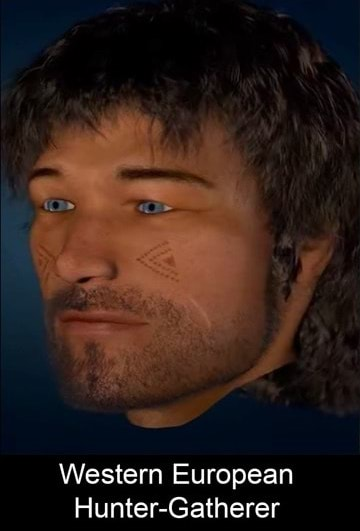
\includegraphics[width=4cm]{whg}
  \caption{This is kind of what angels look like. The angels lack facial hair, however, and have green eyes rather than blue eyes.}
\end{figure}

The Island of Light has a very low population density. There are about 30,000 angels in total living on an island about the size of Maine. The largest town has a population of about 5,000, and is home to the royal family. At the summit of the highest mountain on the island, there is a shrine that only the current king can visit. It is here that he communicates with the God of Gods; see the next section for more information.

\subsection{Deities and Spirits}

Not all of the gods became angels at the end of creation. Among the gods that stayed behind were a small number of major gods and about 8,000 minor gods. The former are referred to as ``deities'' in this document for the sake of disambiguation, but can also be referred to as simply ``gods.'' The latter are referred to as ``spirits.'' The deities never interact with humans directly, but do interact with humans indirectly through phenomena such as volcanoes and the weather, and through the occasional dream or vision. The spirits live in the wild regions of Hom and do interact directly with humans, albeit rarely. The spirits are of a rather antisocial and unpredictable nature, which may explain why they chose not to become angels. Some are benign, while others are more malicious. The deities and spirits, unlike the angels, still retain their original supernatural abilites, including shapeshifting, flying, and so on. Each has its own personality and preferred appearance.

Although the deities never appear to humans, they do occasionally appear to the angels, typically in a humanoid form. The spirits, on the other hand, almost never interact with the angels, preferring to lurk in the wilderness and play tricks on humans that enter their territory.

The most powerful deity is known as the God of Gods, and is suspected of having created all of the other gods. The God of Gods never takes a physical form, and communicates only with the king of the angels, at the shrine atop the highest mountain on the Island of Light.

\section{Geography}

Kalnot is an archipelago in the western part of an ocean known as [ocean name]. It consists of a main island, Kauzei, along with many smaller islands, referred to as the Outer Islands, or \textipa{/k\w oudambe/} in Kalvaszti. (The Kalvaszti term translates literally to ``the Outers.'') Very small islands off the shore of Kauzei are not counted among the Outer Islands.

Kauzei is the southernmost island in Kalnot and is about half the size of Ireland. It constitutes about half of Kalnot's land area and about two-thirds of its population. It also contains the two largest cities in Kalnot: Ruskadai (or Whitecastle) and Kalnofxa (or Greenhaven). Ruskadai is located on the western shore of Kauzei, and Kalnofxa is located in the northeast of Kauzei, on the shore of a large bay. Kalnofxa has a slightly higher population than Ruskadai, but Ruskadai has been the capital of the Kal Empire since its founding.\ [change locations]

\begin{figure}
  \centering
  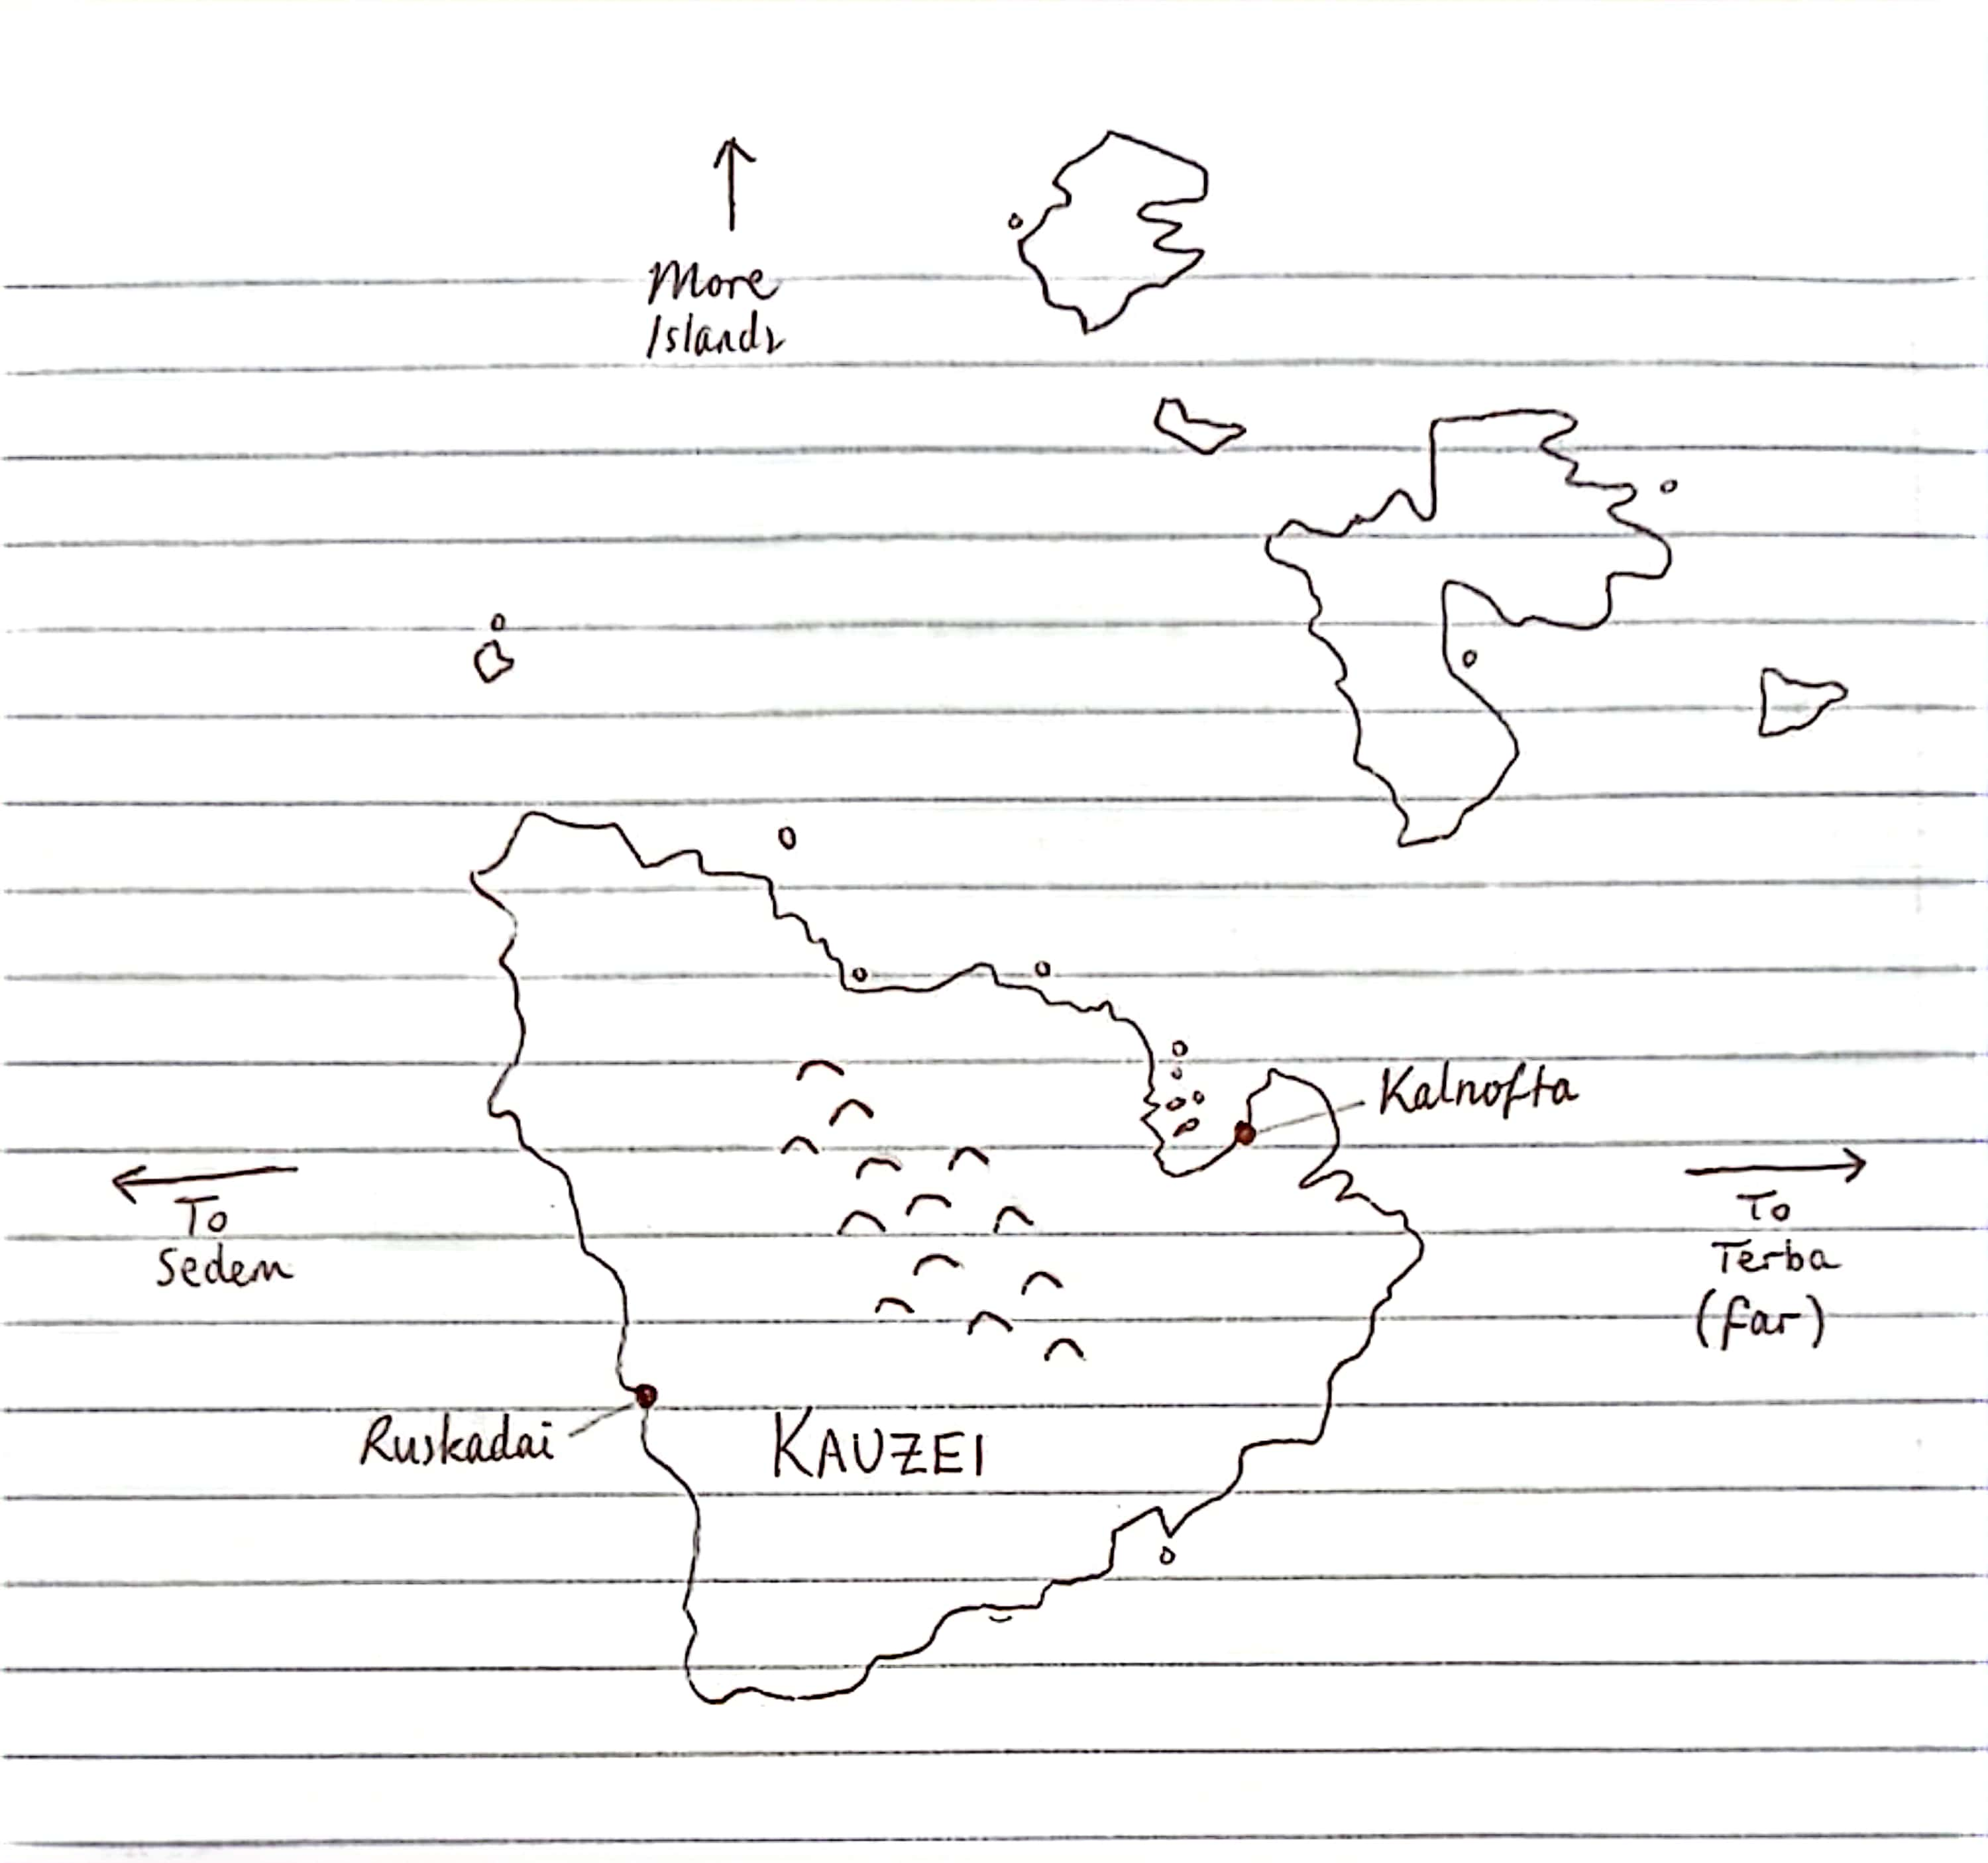
\includegraphics[width=9cm]{kauzei}
  \caption{A hand-drawn map depicting Kauzei and a few other islands, along with the cities of Ruskadai and Kalnofxa (misspelled as ``Kalnofta''). I will update this map at some point.}
\end{figure}

To the west of Kalnot is a continent known as Sedem. It is a fairly small continent, about the size of Australia. Kalnot has had relations with Sedem for thousands of years. In fact, the Kalvaszti language is part of a small language family that originated in Sedem. Kalvaszti is one branch of this family; the other branch consists of three or so languages spoken in the north of Sedem. The languages spoken in the east of Sedem (the part of Sedem closest to Kalnot) are unrelated.

A mountain chain runs east-to-west across the northern part of Sedem. The northern half of the continent is heavily forested, while the southern half consists mostly of sparsely forested grasslands. Most of Sedem, as well as Kalnot, has a temperate or humid continental climate, comparable to Japan, Central Europe, or the eastern United States. Sedem is home to two communities of angels: a group of elusive hunter-gatherers that spend most of their time in the northern mountains, and a group of fishermen that sail from town to town, interacting with and studying the languages and practices of the local humans. The former group arrived in Sedem about 7,000 years ago, while the latter arrived about 500 years ago and will likely depart for another continent in a few centuries.

The societies of Sedem are more technologically advanced than the rest of the world. Humans on Sedem have been farming for around 6,000 years; the only remaining hunter-gatherers are the angels. (Kalnot was inhabited by hunter-gatherers until 2,000 years ago, when the islands were invaded by Proto-Kalvaszti-speaking tribes --- see section \ref{history} for more information.) Sedem is ruled by 22 independent kingdoms.

To the east of [ocean name] is a continent called Terba, which is much larger than Sedem, and much farther than Sedem from Kalnot. Terba extends farther north and farther south than Sedem, and borders the outer darkness at the edge of the world. (``North,'' in the context of Hom, means outward; ``south'' means inward.) The western part of Terba is separated from the rest of the continent by a large mediterranean sea, similar in shape and size to Earth's Mediterranean Sea, but running north-south instead of east-west, and connected to the ocean by a strait at the southern end. So the western part of Terba could be considered an enormous peninsula, on a scale similar to Europe, with the tip at the southern end.

The southern part of this peninsula, along with some land across the sea to the east, is occupied by a large empire. The land to the north is less organized, and is inhabited by farmers and fishermen along the rivers and coasts, and nomadic pastoralists in the interior. Even further north, where the climate is less hospitable, the land is occupied by peoples who live off of hunting, fishing, and reindeer herding.

\section{History of Kalnot}
\label{history}

\section{Kal Society}

\end{document}